\documentclass[
  captions=tableheading,
  bibliography=totoc, 
  titepage=firstiscover,
]{scrartcl}

\usepackage{blindtext} %neuer input

\usepackage{longtable} % Tabellen über mehrere Seiten

\usepackage[utf8]{inputenc} %neuer input

\usepackage{scrhack}

\usepackage[aux]{rerunfilecheck} %Warnung falls nochmal kompiliert werden muss

\usepackage{fontspec} %Fonteinstellungen

\recalctypearea{}

\usepackage[main=ngerman]{babel} %deutsche Spracheinstellung

\usepackage{ragged2e} %neuer input

\usepackage{amsmath, nccmath}

\usepackage{amssymb} %viele mathe Symbole

\usepackage{mathtools} %Erweiterungen für amsmath


\DeclarePairedDelimiter{\abs}{\lvert}{\rvert}
\DeclarePairedDelimiter{\norm}{\lVert}{\rVert}

\DeclarePairedDelimiter{\bra}{\langle}{\rvert}
\DeclarePairedDelimiter{\ket}{\lvert}{\rangle}

\DeclarePairedDelimiterX{\braket}[2]{\langle}{\rangle}{
#1 \delimsize| #2
}

\NewDocumentCommand \dif {m}
{
\mathinner{\symup{d} #1}
}


\usepackage[
  math-style=ISO,
  bold-style=ISO,
  sans-style=italic,
  nabla=upright,
  partial=upright,
  warnings-off={
    mathtools-colon,
    mathtools-overbracket,
  },
]{unicode-math}

\setmathfont{Latin Modern Math}
\setmathfont{XITS Math}[range={scr, bfscr}]
\setmathfont{XITS Math}[range={cal, bfcal}, StylisticSet=1]


\usepackage[
  locale=DE,
  separate-uncertainty=true,
  per-mode=reciprocal,
  output-decimal-marker={,},
]{siunitx}

\usepackage[autostyle]{csquotes} %richtige Anführungszeichen

\usepackage{xfrac}

\usepackage{float}

\floatplacement{figure}{htbp}

\floatplacement{table}{htbp}

\usepackage[ %floats innerhalb einer section halten
  section,   %floats innerhalb er section halten
  below,     %unterhalb der Section aber auf der selben Seite ist ok
]{placeins}

\usepackage[
  labelfont=bf,
  font=small,
  width=0.9\textwidth,
]{caption}

\usepackage{subcaption} %subfigure, subtable, subref

\usepackage{graphicx}

\usepackage{grffile}

\usepackage{booktabs}

\usepackage{microtype} %Verbesserungen am Schriftbild

\usepackage[
backend=biber,
]{biblatex}

\addbibresource{../lit.bib}

\usepackage[ %Hyperlinks im Dokument
  german,
  unicode,
  pdfusetitle,
  pdfcreator={},
  pdfproducer={},
]{hyperref}

\usepackage{bookmark}

\usepackage[shortcuts]{extdash}

%\usepackage{warpcol}


\begin{document}
    \title{V311 Der Hall-Effekt}
    \author{  
    Tobias Rücker\\
    \texorpdfstring{\href{mailto:tobias.ruecker@tu-dortmund.de}{tobias.ruecker@tu-dortmund.de}
    \and}{,} 
    Paul Störbrock\\
    \texorpdfstring{\href{mailto:paul.stoerbrock@tu-dortmund.de}{paul.stoerbrock@tu-dortmund.de}}{}
    }
    \date{Durchführung: 21.01.20, Abgabe: 28.01.20 \vspace{-4ex}}
\maketitle
\center{\Large Versuchsgruppe: \textbf{42}}
\thispagestyle{empty}

\newpage
\tableofcontents
\thispagestyle{empty}
\newpage

% Ziel %%%%%%%%%%%%%%%%%%%%%%%%%%%%%%%%%%%%%%%%%%%%%%%%%%%%%%%%%%%%%%%%%%%%%%%%%%%%%%%%%%%%%%%%%%%%%%%%%%%%%%%%%%%%%%%%%%%%%%%%%%%%%%%%%%%%%%%%%%%%%%%%%%%%%%%%%%%%%%%%%%%%%%%%%%%%%%%%%%%%%%%%%%%%%%%%%%%%%%%%%%%%%%%%%

\setcounter{page}{1}
\section{Ziel} \label{sec:1}\justifying
In der heutigen Zeit bilden Kenntnisse zur elektrischen Leitfähigkeit von Metallen eine entscheidende Rolle.
Die meiste Technick von heute benötigt Kenntnisse über die Leitfähigkeit von verschiedenen
Materialien wie Metallen. Eine effiziente Möglichkeit zur Untersuchung der verschiedenen
elektrischen Leitungseigenschaften bildet der Versuch zum Hall-Effekt.

% Theorie %%%%%%%%%%%%%%%%%%%%%%%%%%%%%%%%%%%%%%%%%%%%%%%%%%%%%%%%%%%%%%%%%%%%%%%%%%%%%%%%%%%%%%%%%%%%%%%%%%%%%%%%%%%%%%%%%%%%%%%%%%%%%%%%%%%%%%%%%%%%%%%%%%%%%%%%%%%%%%%%%%%%%%%%%%%%%%%%%%%%%%%%%%%%%%%%%%

\section{Theorie} \label{sec:2}\justifying
Kristalline Festkörper haben die Eigenschaft, dass deren Valenzelektronen ein System  bilden.
Valenzelektronen sind dabei die Elektronen in der äußersten Schale des Atoms. 
Für diese Elektronen gilt das Pauli-Prinzip, was bedeutet, dass jedes Elektron
in diesem System einen anderen Quantenzustand annimmt. Daraus folgt, dass alle Elektronen
eine leicht verschiedene Energie haben. Dadurch entstehen Energiebänder in der
Elektronenhülle. Diese Energiebänder können sich überlappen
oder eine Lücke bilden, welche als verbotene Zone bezeichnet wird, sofern sie eine endliche 
Breite hat. Eine weitere Folge des Pauli-Prinzips ist, dass sich nur eine endliche Anzahl
an Elektronen auf den Energiebändern befinden kann. \\
Elektronen auf besetzten Bändern leisten keinen Beitrag zur elektrischen Leitfähigkeit.
Bei Metallen führt daher das höchste teils nicht besetzte Band zu ihrer elektrischen
Leitfähigkeit. Die Elektronen auf diesem Band werden als Leitunselektronen bezeichnet.
Die Anzahl der freien Leitungselektronen in einem Volumen $V$ lässt sich dabei über die Hallspannung
berechnen: \cite{V311}
\begin{align}
    U_H =- \frac{1}{n e_0} \frac{B \cdot I_q}{d}. \label{eq:1}
\end{align}
Die Hallspannung beschreibt dabei eine Messgröße des Halleffekts. Bei diesem wird 
ein Querstrom $I_q$ durch eine Leiterplatte der Dicke $d$ geleitet, während die
Leiterplatte sich in einem homogenen Magnetfeld senkrecht zur Probe befindet. 
Durch das Magnetfeld wirkt auf die Elektronen die Lorentzkraft, welche dazu führt,
dass die Elektronen durch die Auslenkung ein elektrisches Feld aufbauen. Die sich, nach
dem Kompensieren der Lorentzkraft mit der des elektrischen Feldes, einstellende 
Spannung wird Hallspannung genannt. Das $n$ aus Formel \eqref{eq:1} bescheibt dabei die Anzahl
der freien Ladungsträger in der Leiterplatte. Die Konstante $e_0$ beschreibt hier die Ladung des Elektrons.
Beide Parameter bilden zusammen die Hallkonstante: \cite{grosse2016physikalische}
\begin{align}
    R_H = \frac{1}{n e_0} \label{eq:2}
\end{align}
Um die Anzahl der freien Elektronen für ein Atom zu bestimmen, muss $n$ auf die Anzahl der Atome
im Volumen normiert werden:
\begin{align}
    z = \frac{n}{\frac{N}{V}} \label{eq:3}
\end{align}
Der Nenner von z lässt sich dabei über die Dichte bestimmen
\begin{subequations}
\begin{align}
    \rho = \frac{m}{V} \label{eq:4a} \\
    \intertext{wobei sich $m$ mit
    }
    m =N \cdot A_u \cdot u \label{eq:4b} \\
    \intertext{beschreiben lässt. Dabei bildet $A_u$ die relative Atommasse, während u die atomare Masseneinheit darstellt.
    Diese ergibt für $\sfrac{N}{V}$
    }
    \frac{N}{V}= \frac{\rho}{A_u \cdot u}.\label{eq:4c} \\
    \intertext{ Dadurch ergibt sich für $z$
    }
    z=\frac{n \cdot A_u \cdot u}{\rho}. \label{eq:4d}
\end{align}
\end{subequations}
Die Leitungselektronen bewegen sich im Gitterverband dabei wie Teilchen in einem idealen Gas.
Die ungeordnete Bewegung dieser Teilchen führt zu Zusammenstößen mit Fremdatomen und anderen
strukturellen Defiziten. Durch diese Zusammenstöße kommt es zu einer Streuung der
Elektronen in eine zufällige Richtung. Um die Geschwindigkeit der Elektronen in 
Richtung des E-Feldes zu definieren, wird eine neue Größe, nämlich die mittlere Driftgeschwindigkeit
$\overline{v} _d$, eingeführt. Diese ist über die Stromdichte j folgendermaßen definert: \cite{V311}
\begin{align}
    j = -n \, \overline{v} _d\, e_0 \label{eq:5}
\end{align}
Durch Umschreiben der Driftgeschwindigkeit lässt sich eine weitere wichtige Größe einführen,
die mittlere Flugzeit $\overline{\tau}\,$: \cite{V311}
\begin{align}
    j = \frac{1}{2}\frac{e_0^2}{m_0} n \overline{\tau} E \label{eq:6}
\end{align}
Dabei ist $E$ der Betrag des E-Feldes und $m_0$ die Ruhemasse des Elektrons.
Berechnen lässt sich die mittlere Flugzeit dabei über die Formel \cite{V311}
\begin{align}
\varrho = 2 \frac{m_0}{e_0^2}\frac{1}{n \overline{\tau}}. \label{eq:7}
\end{align}
Eine weitere wichtige mikroskopische Größe stellt die Totalgeschwindigkeit $\abs{v}$ dar.
Diese beschreibt die Geschwindigkeit, welche durch die thermische Bewegung der einzelnen
Bausteine des Kristalls hervorgerufen wird. Aufgrund des Pauli-Prinzips lässt sich
die Energieverteilung nicht durch eine Maxwell-Boltzmann-Verteilung darstellen, 
sondern durch eine Fermi-Dirac-Verteilung \cite{V311}
\begin{align}
    f(E) dE=\frac{1}{e^{\frac{E-E_F}{kT}}+1}dE . \label{eq:8}
\end{align}
Der Parameter $E_F$ bedeutet die Fermi-Energie. Sie beschreibt den Energiewert
der Elektronen mit der meisten Energie aufrgrund des Pauli-Prinzips am absoluten
Nullpunkt. Die Fermi-Energie sieht als Formel folgendermaßen aus: \cite{V311}
\begin{align}
    E_F = \frac{h^2}{2 m_0} \sqrt[3]{\left(\frac{3}{8 \pi}n \right)^2} \label{eq:9}
\end{align}
Mit \eqref{eq:9} lässt sich die Totalgeschwindigkeit $\abs{v} $ abschätzen, da nur die
Elektronen mit $E\approx E_F$ einen Beitrag zur Leitfähigkeit leisten \cite{V311}
\begin{align}
    \abs{v} \approx \sqrt{\frac{2 E_F}{m_0}}. \label{eq:10}
\end{align}
Aus $\overline{\tau}$ und $\abs{v} $ lässt sich eine weitere Größe berechnen, die mittlere
freie Weglänge: \cite{V311}
\begin{align}
    \overline{l} = \overline{\tau} \abs{v} \label{eq:11} \\
    \intertext{Durch das Einsetzen von Formel \eqref{eq:10} ergibt sich dann:}
    \overline{l} \approx \overline{\tau} \sqrt{\frac{2 E_F}{m_0}} \label{eq:12}
\end{align}
Die freie Weglänge beschreibt dabei den Weg, den ein Elektron zwischen zwei Zusammenstößen
im Mittel zurücklegt.
Aus der mittleren Flugzeit lässt noch die Beweglichkeit $\mu$ ableiten \cite{V311}
\begin{align}
    \vec{\overline{v}} _d = \mu \vec{E} \label{eq:13}.
\end{align}
Die Beweglichkeit beschreibt hier, wie störfrei sich die Elektronen in dem Metall 
ausbreiten können.\\
Bei überlappenden Energiebändern kann es passieren, dass Elektronen vom nieder- ins höherenergetische
Band übergehen. Dann entsteht eine Leerstelle im niederen Band, welche als Loch bezeichnet wird.
Diese werden von einem elektrische Feld beeinflusst und verhalten sich ähnlich einer positiven Ladung.
Sie sind damit ein Teil des Hall-Effekts, bei dem die Hall-Spannung allerdings das 
Vorzeichen wechselt. Dies nennt     man den anomalen Hall-Effekt.

% Fehlerrechnung %%%%%%%%%%%%%%%%%%%%%%%%%%%%%%%%%%%%%%%%%%%%%%%%%%%%%%%%%%%%%%%%%%%%%%%%%%%%%%%%%%%%%%%%%%%%%%%%%%%%%%%%%%%%%%%%%%%%%%%%%%%%%%%%%%%%%%%%%%%%%%%%%%%%%%%%%%%%%%%%%%%%%%%%%%%%%%%%%%%%%%%%%%%%%%%%%%%%%%

\section{Fehlerrechnung} \label{sec:3}\justifying

Für die Berechnung von Messunsicherheiten werden in diesem Protokoll folgende Formeln
verwendet:
\begin{subequations} \label{eq:14}
\begin{align} 
\intertext{Zur Bestimmung eines Mittelwertes wird folgende Formel benutzt:
}
    \overline{x} &= \frac{1}{N}\sum_{i=1}^{N} x_i \label{eq:14a}
\intertext{Zur Bestimmung der Messunsicherheit bei Mittelwerten wird mit der Formel
}
    \Delta\overline{x} &= \frac{1}{\sqrt{N}} \sqrt{\frac{1}{1-N} \sum_{i=1}^{N} (x_i - \overline{x})^2} \label{eq:14b},
\intertext{gearbeitet und die Gaußsche Fehlerfortpflanzung wird mit
}
    \Delta f &= \sqrt{\sum_{i=1}^{N} \left( \frac{\delta f}{\delta x_i} \right)^2 \cdot (\Delta x_i)^2} \label{eq:14c}
\intertext{berechnet. Um Ausgleichsgeraden und ihre Parameter zu bestimmen, werden folgende Formeln verwendet:
}
    y &= m \cdot x + b \label{eq:14d} \\ 
    m &= \frac{\overline{xy} - \overline{x} \cdot \overline{y}}{\overline{x^2} - {\overline{x}}^2} \label{eq:14e}\\
    b &= \frac{\overline{y} \cdot \overline{x^2} - \overline{xy} \cdot \overline{x}}{\overline{x^2} - {\overline{x}}^2} \label{eq:14f}
\end{align}
\end{subequations}
\newpage

% Versuchsaufbau + Versuchsdurchführung %%%%%%%%%%%%%%%%%%%%%%%%%%%%%%%%%%%%%%%%%%%%%%%%%%%%%%%%%%%%%%%%%%%%%%%%%%%%%%%%%%%%%%%%%%%%%%%%%%%%%%%%%%%%%%%%%%%%%%%%%%%%%%%%%%%%%%%%%%%%%%%%%%%%%%%%%%%%%%%%%%%%%%%%%%%%%%%%%%%%%%%%%%%%%%%%%%

\section{Versuchsaufbau und Versuchsdurchführung} \label{sec:4}\justifying
Benötigt werden: \textit{Ein Eisenjoch, zwei Spulen, zwei Magnetschuhe, drei Leiterplatten, drei Materialproben , 
ein digitales Multimeter, zwei Generatoren , jeweils drei Spulen aus dem Material der einzelnen Proben,
eine Hall-Sonde, eine digitale Mikrometerschraube
und sieben Experimentierkabel.}

\flushleft{Zu\;}\justifying Beginn wird das Eisenjoch durch beide Spulen geführt. An beiden Enden des Eisenjochs werden nun die Magnetschuhe
angebracht. Sobald der Elektromagnet aufgebaut ist, werden die beiden Spulen in Reihe geschaltet und an den einen Generator angeschlossen. Nun wird eine Hall-Sonde an einem Stativ befestigt und zwischen die Magnetschuhe gestellt, um
die Hysterese des Magnetfelds zu bestimmen. Dafür wird der Strom sukzessiv 
, bis eine festgelegte Spannung an den Spulen anliegt. Für jede Erhöhung des Stroms wird die Stärke
des Magnetfelds mit der Hall-Sonde abgelesen. Ist die festgelegte Spannung erreicht, wird der selbe Prozess wiederholt während der Strom reduziert
wird. 

\flushleft{Sind\;}\justifying die Messwerte der Hysterese bestimmt, wird die Hall-Sonde entfernt und eine Materialprobe auf der 
Leiterplatte zwischen den Magnetschuhen befestigt. Anschließend wird die Leiterplatte wie folgt an dem Multimeter und Generator angeschlossen:

\begin{figure}[H]
    \centering
    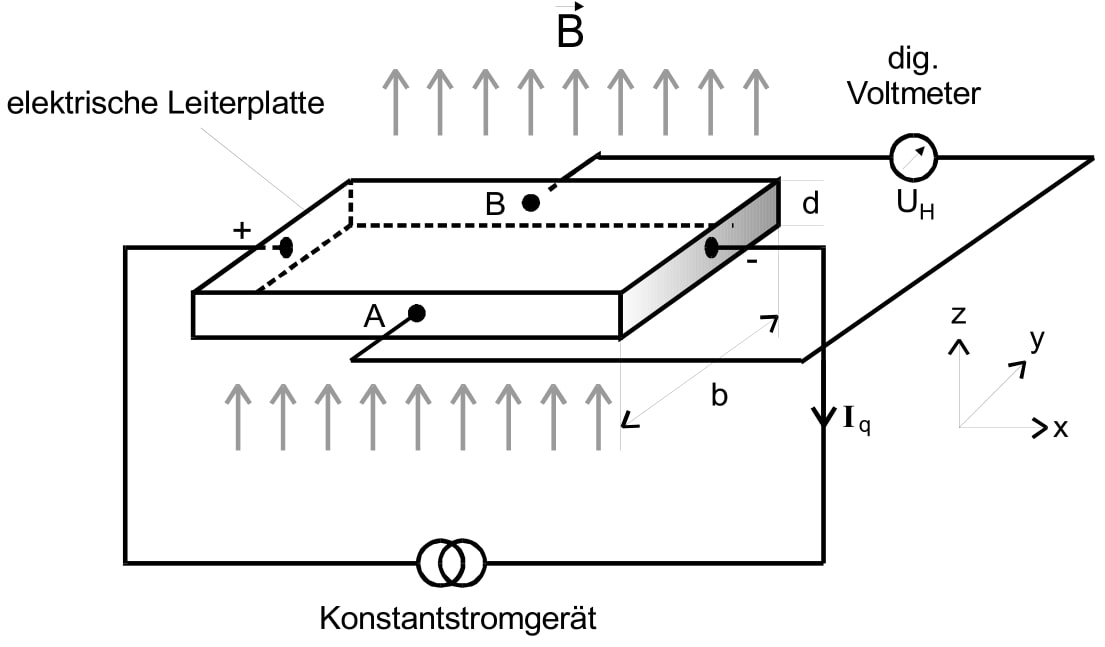
\includegraphics[width=\linewidth]{./images/leiterplatte.jpg}
    \caption{Aufbau der Leiterplatte \cite{V311}}
    \label{fig:1}
\end{figure}

\flushleft{Nun\;}\justifying werden die Messwerte der Hallspannung aufgenommen. Dafür werden zwei Messreihen angefertigt. Es wird einmal 
der Querstrom $I_Q$ konstant gehalten und einmal der Strom $I_B$, welcher durch die Spulen fließt und das Magnetfeld
induziert. Wenn der Querstrom konstant gehalten wird, wird der Strom $I_B$ in 
gleichmäßigen Schritten erhöht, sodass zehn Messwerte aufgenommen werden können. Ähnlich wird beim konstanten
Magnetfeld verfahren. Hier wird $I_Q$ in gleichmäßigen Schritten hochgedreht. Dabei wird der Strom
bis zur maximalen Angabe für die Leiterplatte erhöht.

\flushleft{Anschließend\;}\justifying wird die Foliendicke und der Drahtdurchmesser der Probe mit einer Mikrometerschraube gemessen. Der Widerstand wird 
mit einer Spule des jeweiligen Metalls bestimmt. Dafür wird die Spule mit dem digitalen Multimeter verbunden und
der Widerstand auf dem Display ausgegeben.


% Auswertung %%%%%%%%%%%%%%%%%%%%%%%%%%%%%%%%%%%%%%%%%%%%%%%%%%%%%%%%%%%%%%%%%%%%%%%%%%%%%%%%%%%%%%%%%%%%%%%%%%%%%%%%%%%%%%%%%%%%%%%%%%%%%%%%%%%%%%%%%%%%%%%%%%%%%%%%%%%%%%%%%%%%%%%%%%%%%%%%%%%%%%%%%%%%%%%%%%

\section{Auswertung} \label{sec:5}

\subsection{Messwerte} \label{sec:5.1}

\flushleft{Es\;}\justifying werden die drei Materialien Kupfer, Silber und Zink verwendet. 
 Die gemessenen Maße der Folien und Drähte, sowie der Widerstände der Materialien lauten:

\begin{table}[H]
\centering
    \begin{tabular}{l r r r}
    \toprule
        \multicolumn{1}{c}{} & \multicolumn{1}{c}{Kupfer} & \multicolumn{1}{c}{Silber} & \multicolumn{1}{c}{Zink}\\
        \cmidrule(lr{0,5em}){1-4}
        Foliendicke $d$        & \text{\input{d_Cu_Folie.tex}}   & \text{\input{d_Ag_Folie.tex}}   & \text{\input{d_Zn_folie.tex}}\\
        Drahtdurchmesser    & \text{\input{d_Cu_Draht.tex}}   & \text{\input{d_Ag_Draht.tex}}   & \text{}\\
        Drahtlänge $l$         & \text{\input{l_Cu.tex}}         & \text{\input{l_Ag.tex}}         & \text{}\\
        Widerstand $R$         & \text{\input{R_Cu.tex}}         & \text{\input{R_Ag.tex}}         & \text{}\\
        Dichte  $\rho$            & \text{\input{varrho_Cu.tex}}    & \text{\input{varrho_Ag.tex}}    & \text{\input{varrho_Zn.tex}}\\
        Relative Atommasse $A_u$      & \text{\input{atom_mass_Cu.tex}} & \text{\input{atom_mass_Ag.tex}} & \text{\input{atom_mass_Zn.tex}}\\
        \bottomrule
    \end{tabular}
\caption{Messwerte für den Spezifischen Widerstand}
\label{tab:1}
\end{table}

\flushleft{Mithilfe\;}\justifying der Messwerten aus Tabelle \ref{tab:1} lässt sich der spezifische Widerstand $\varrho = R \cdot \sfrac{A}{l}$
der einzelnen Materialien bestimmen. Hier wird der Literaturwert des spezifischen Widerstands für Zink \cite{SpWiderstand_Zn} genommen, da für 
Zink keine Spule und kein Draht zur Verfügung stand. Damit lauten die spezifischen Widerstände:
\begin{subequations} \label{eq:15}
\begin{align}
    \varrho_{Cu} &= \text{\input{rho_Cu.tex}} \label{eq:15a}\\
    \varrho_{Ag} &= \text{\input{rho_Ag.tex}} \label{eq:15b}\\
    \varrho_{Zn} &= \text{\input{rho_Zn.tex}} \label{eq:15c}
\end{align}
\end{subequations}

% Hysterese ===============================================================================================================================================================================================================
\subsection{Hysterese} \label{sec:5.2}

\flushleft{Die\;}\justifying folgende Tabelle \ref{tab:2} gibt die Messwerte des Magnetfeldes für einen steigenden Strom (links) und einem 
sinkenden Strom (rechts) wieder. 

\begin{table}[H]
    \centering
    \input{Hysterese_table.tex}
    \caption{Hysterese des Magnetfelds}
    \label{tab:2}
\end{table}

\flushleft{Mithilfe\;}\justifying der Messwerte aus Tabelle \ref{tab:2} lässt sich der Graph \ref{fig:2} erstellen. Der folgende Graph wird 
mit dem Phython Befehl np.polyfit() \cite{numpy} und der Formel \eqref{eq:14d} $y = mx + b$ erstellt. Die Parameter $m$ und $b$ werden mit 
den Formeln \eqref{eq:14e} und \eqref{eq:14f} bestimmt und lauten:
\begin{subequations}
\begin{align}
    m_{auf} &= \text{\input{m_hyauf.tex}} \label{eq:16a}\\
    b_{auf} &= \text{\input{b_hyauf.tex}} \label{eq:16b}\\
    m_{ab}  &= \text{\input{m_hyab.tex}}  \label{eq:16c}\\
    b_{ab}  &= \text{\input{b_hyab.tex}}  \label{eq:16d}
\end{align}
\end{subequations}

\begin{figure}[H]
\centering
\includegraphics[width=0.75\linewidth]{./build/plothy.pdf}
\caption{Hysteresekurve}
\label{fig:2}
\end{figure}

% Kupfer ===============================================================================================================================================================================================================
\subsection{Kupfer} \label{sec:5.3}

\flushleft{Die\;}\justifying folgende Tabelle \ref{tab:3} gibt die Messwerte der Hallspannung $U_H$ bei variierendem Querstrom $I_Q$ oder Magnetfeld
$I_B$ für Kupfer wieder:

\begin{table}[H]
    \centering
    \input{Cu_table.tex}
    \caption{Hallspannung $U_H$ von Kupfer}
    \label{tab:3}
\end{table}

\flushleft{Die\;}\justifying folgenden Graphen \ref{fig:3a} und \ref{fig:3b} werden mit den jeweiligen Messwerten aus Tabelle \ref{tab:3} 
angefertigt. Außerdem lauten die relevanten Parameter: 
\begin{subequations} \label{eq:17}
\begin{align}
    m_{a)} &= \text{\input{m_Cu_IQ.tex}} \label{eq:17a}\\
    b_{a)} &= \text{\input{b_Cu_IQ.tex}} \label{eq:17b}\\
    m_{b)} &= \text{\input{m_Cu_IB.tex}} \label{eq:17c}\\
    b_{b)} &= \text{\input{b_Cu_IB.tex}} \label{eq:17d}
\end{align}
\end{subequations}

\begin{figure}[H]
\begin{subfigure}{0.495\linewidth}
\centering
\includegraphics[width=\linewidth]{./build/plotCu_IB.pdf}
\caption{Hallspannung bei konstantem Querstrom}
\label{fig:3a}
\end{subfigure}
\begin{subfigure}{0.495\linewidth}
\centering
\includegraphics[width=\linewidth]{./build/plotCu_IQ.pdf}
\caption{Hallspannung bei konstantem B-Feld}
\label{fig:3b}
\end{subfigure}
\caption{Hallspannungen für Kupfer}
\label{fig:3}
\end{figure}

\subsubsection{Konstanter Querstrom} \label{sec:5.3.1}
 
\flushleft{Die\;}\justifying Ladungsträger pro Volumen $n$ lassen sich mit der Formel \eqref{eq:1} bestimmen. Dafür wird das Magnetfeld $B$
benötigt, welches sich mit den Steigung $m_{auf}$ \eqref{eq:16a} oder $m_{ab}$ \eqref{eq:16c} des Graphen \ref{fig:2} bestimmen lässt, da 
Das B-Feld aus der Geradengleichung $B = m_{auf/ab} \cdot I + b_{auf/ab}$ folgt. Wird der Wert mit dem dazugehörigen Werten aus
Tabellen \ref{tab:1} und \ref{tab:2} in Formel \eqref{eq:1} eingesetzt, folgt für $n$:
\begin{align}
    n_{Cu} = \text{\input{n_Cu_IB.tex}} \label{eq:18}
\end{align}

\flushleft{Mithilfe\;}\justifying von $n$ lässt sich die Zahl der Ladungsträger pro Volumen $z$ mit der Formel \eqref{eq:4d} bestimmen. 
Mit den Werten aus Tabelle \ref{tab:1} und $n_{Cu}$ \eqref{eq:18} folgt für $z$:
\begin{align}   
    z_{Cu} = \frac{n \cdot A_u \cdot u}{\rho} = \text{\input{z_Cu_IB.tex}} \label{eq:19}
\end{align}

\flushleft{Die\;}\justifying Hallkonstante für Kupfer wird mithilfe der Formel \eqref{eq:2} berechnet. Hier wird das zuvor berechnete $n_{Cu}$ 
\eqref{eq:18} eingesetzt. Daraus folgt die Hallkonstante:
\begin{align}
    R_{H,Cu} = \text{\input{AH_Cu_IB.tex}} \label{eq:20}
\end{align}

\flushleft{Die\;}\justifying mittlere Flugzeit $\overline{\tau}$ berechnet sich mit der Formel \eqref{eq:7}. Die Konstanten $e_0$ und $m_0$ und 
der spezifische Widerstand $\varrho_{Cu}$ \eqref{eq:15a} werden in Formel \eqref{eq:7} eingesetzt, nachdem diese nach $\overline{\tau}$ umgestellt 
wurde. Daraus folgt für $\overline{\tau}\,$:
\begin{align}
        \overline{\tau}_{Cu} &= 2\frac{m_0}{e_0^2}\frac{1}{n\varrho} = \text{\input{tau_Cu_IB.tex}} \label{eq:21}
    \intertext{
        Für die mittlere Driftgeschwindigkeit $\overline{v}_d$ wird die Formel \eqref{eq:5} umgestellt. Auch hier wird das zuvor berechnete
    $n_{Cu}$ \eqref{eq:18} eingesetzt, woraus folgt:
    }
        \overline{v}_{d,Cu} &= \frac{-j}{n e_0} = \text{\input{v_d_Cu_IB.tex}} \label{eq:22}
    \intertext{
        Mit $\overline{\tau}$ lässt sich außerdem der Betrag des elektrischen Feldes $E$ mithilfe der Formel \eqref{eq:6} berechnen.
    Für $E$ folgt:
    }
        E &= 2\frac{j}{n \overline{\tau}}\frac{m_0}{e_0^2} \label{eq:23}
    \intertext{
        Mit dem Betrag des E-Feldes lässt sich nun die Beweglichkeit der Elektronen $\mu$ bestimmen. Dafür wird die Formel \eqref{eq:13}
    nach $\mu$ umgestellt und die Werte für $\overline{v}_{d,Cu}$ \eqref{eq:21} und $E$ \eqref{eq:23} eingesetzt:
    }
        \mu_{Cu} &= \frac{\overline{v}_{d,Cu}}{E} = \text{\input{mu_Cu_IB.tex}} \label{eq:24}
    \intertext{
        Um die mittlere Weglänge $\overline{l}$ zu bestimmen, wird zuerst die Fermi-Energie $E_F$ nach Formel \eqref{eq:9} und die
        durch $E_F$ bestimmte absolute Geschwindigkeit $\abs{v}$ berechnet.
        Daraus folgt für $E_F$:
    }
        E_F &= \frac{h^2}{2 m_0} \sqrt[3]{\left(\frac{3}{8 \pi}n \right)^2} \label{eq:25}
    \intertext{
        Wird $E_F$ nun in Formel \eqref{eq:10} eingesetzt, folgt für die absolute Geschwindigkeit:
    }
        \abs{v}_{Cu} &\approx \sqrt{\frac{2 E_F}{m_0}} = \text{\input{v_Cu_IB.tex}} \label{eq:26}
    \intertext{
        Mit der absoluten Geschwindigkeit lässt sich $\overline{l}$ approximieren als:   
    }
        \overline{l}_{Cu} &\approx \overline{\tau}\sqrt{\frac{2 E_F}{m_0}} = \text{\input{l_Cu_IB.tex}} \label{eq:27}
\end{align}

\subsubsection{Konstantes B-Feld} \label{sec:5.3.2}

\flushleft{Die\;}\justifying Werte für ein konstantes B-Feld werden analog zu Abschnitt \ref{sec:5.3.1} berechnet. 
Die Ergebnisse lauten wie folgt:

\begin{table}[H]
\centering
    \begin{tabular}{l r l}
    \toprule
        Ladungsträger pro Volumen               &$n_{Cu}$               = & \text{\input{n_Cu_IQ.tex}}  \\
        Zahl der Ladungsträger pro Volumen      &$z_{Cu}$               = & \text{\input{z_Cu_IQ.tex}}  \\
        Hallkonstante                           &$R_{H,Cu}$             = & \text{\input{AH_Cu_IQ.tex}} \\
        Mittlere Flugzeit                       &$\overline{\tau}_{Cu}$ = & \text{\input{tau_Cu_IQ.tex}}\\
        Mittlere Driftgeschwindigkeit           &$\overline{v}_{d,Cu}$  = & \text{\input{v_d_Cu_IQ.tex}}\\
        Beweglichkeit                           &$\mu_{Cu}$             = & \text{\input{mu_Cu_IQ.tex}} \\
        Totalgeschwindigkeit                    &$\abs{v}_{Cu}$         = & \text{\input{v_Cu_IQ.tex}}  \\
        Mittlere freie Weglänge                 &$\overline{l}_{Cu}$    = & \text{\input{l_Cu_IQ.tex}}  \\
        \bottomrule
    \end{tabular}
\caption{Werte für Kupfer mit konstantem B-Feld}
\label{tab:4}
\end{table}

% Silber ===============================================================================================================================================================================================================
\subsection{Silber} \label{sec:5.4}

\flushleft{In\;}\justifying der folgenden Tabelle \ref{tab:5} sind Hallspannung $U_H$ und Strom $I$ für Silber aufgetragen. Auch hier ist auf der
linken Seite der Querstrom konstant und auf der rechten Seite das Magnetfeld. 
 
\begin{table}[H]
    \centering
    \input{Ag_table.tex}
    \caption{Hallspannung $U_H$ von Silber}
    \label{tab:5}
\end{table}

\flushleft{Die\;}\justifying folgenden zwei Graphen \ref{fig:4a} und \ref{fig:4b} werden mit den Messwerten aus Tabelle \ref{tab:5}
und den relevanten Parameter $m$ und $b$
\begin{subequations} \label{eq:28}
\begin{align}
    m_{a)} &= \text{\input{m_Ag_IQ.tex}} \label{eq:28a}\\
    b_{a)} &= \text{\input{b_Ag_IQ.tex}} \label{eq:28b}\\
    m_{b)} &= \text{\input{m_Ag_IB.tex}} \label{eq:28c}\\
    b_{b)} &= \text{\input{b_Ag_IB.tex}} \label{eq:28d}
\end{align}
\end{subequations}

\begin{figure}[H]
\begin{subfigure}{0.495\linewidth}
\centering
\includegraphics[width=\linewidth]{./build/plotAg_IB.pdf}
\caption{Hallspannung bei konstantem Querstrom}
\label{fig:4a}
\end{subfigure}
\begin{subfigure}{0.495\linewidth}
\centering
\includegraphics[width=\linewidth]{./build/plotAg_IQ.pdf}
\caption{Hallspannung bei konstantem B-Feld}
\label{fig:4b}
\end{subfigure}
\caption{Hallspannungen für Silber}
\label{fig:4}
\end{figure}

\subsubsection{Konstanter Querstrom} \label{sec:5.4.1}

\flushleft{Die\;}\justifying Werte für einen konstanten Querstrom werden analog zu Abschnitt \ref{sec:5.3.1} berechnet. 
Die Ergebnisse lauten wie folgt:

\begin{table}[H]
\centering
    \begin{tabular}{l r l}
    \toprule
        Ladungsträger pro Volumen               &$n_{Ag}$               = & \text{\input{n_Ag_IB.tex}}  \\
        Zahl der Ladungsträger pro Volumen      &$z_{Ag}$               = & \text{\input{z_Ag_IB.tex}}  \\
        Hallkonstante                           &$R_{H,Ag}$             = & \text{\input{AH_Ag_IB.tex}} \\
        Mittlere Flugzeit                       &$\overline{\tau}_{Ag}$ = & \text{\input{tau_Ag_IB.tex}}\\
        Mittlere Driftgeschwindigkeit           &$\overline{v}_{d,Ag}$  = & \text{\input{v_d_Ag_IB.tex}}\\
        Beweglichkeit                           &$\mu_{Ag}$             = & \text{\input{mu_Ag_IB.tex}} \\
        Totalgeschwindigkeit                    &$\abs{v}_{Ag}$         = & \text{\input{v_Ag_IB.tex}}  \\
        Mittlere freie Weglänge                 &$\overline{l}_{Ag}$    = & \text{\input{l_Ag_IB.tex}}  \\
        \bottomrule
    \end{tabular}
\caption{Werte für Silber mit konstantem Querstrom}
\label{tab:6}
\end{table}

\subsubsection{Konstantes B-Feld} \label{sec:5.4.2}

\flushleft{Die\;}\justifying Werte für ein konstantes B-Feld werden analog zu Abschnitt \ref{sec:5.3.1} berechnet. 
Die Ergebnisse lauten wie folgt:

\begin{table}[H]
\centering
    \begin{tabular}{l r l}
    \toprule
        Ladungsträger pro Volumen               &$n_{Ag}$               = & \text{\input{n_Ag_IQ.tex}}  \\
        Zahl der Ladungsträger pro Volumen      &$z_{Ag}$               = & \text{\input{z_Ag_IQ.tex}}  \\
        Hallkonstante                           &$R_{H,Ag}$             = & \text{\input{AH_Ag_IQ.tex}} \\
        Mittlere Flugzeit                       &$\overline{\tau}_{Ag}$ = & \text{\input{tau_Ag_IQ.tex}}\\
        Mittlere Driftgeschwindigkeit           &$\overline{v}_{d,Ag}$  = & \text{\input{v_d_Ag_IQ.tex}}\\
        Beweglichkeit                           &$\mu_{Ag}$             = & \text{\input{mu_Ag_IQ.tex}} \\
        Totalgeschwindigkeit                    &$\abs{v}_{Ag}$         = & \text{\input{v_Ag_IQ.tex}}  \\
        Mittlere freie Weglänge                 &$\overline{l}_{Ag}$    = & \text{\input{l_Ag_IQ.tex}}  \\
        \bottomrule
    \end{tabular}
\caption{Werte für Silber mit konstantem B-Feld}
\label{tab:7}
\end{table}

% Zink ===============================================================================================================================================================================================================
\subsection{Zink} \label{sec:5.5}

\flushleft{Die\;}\justifying folgende Tabelle \ref{tab:8} enthällt die Messwerte der Hallspannung $U_H$ und des dazugehörigen Stroms von Zink.
Wie auch in Sektion \ref{sec:5.4} ist auf der linken Seite der Querstrom konstant gehalten und auf der rechten Seite das Magnetfeld.

\begin{table}[H]
    \centering
    \input{Zn_table.tex}
    \caption{Hallspannung $U_H$ von Zink}
    \label{tab:8}
\end{table}

\flushleft{Mit\;}\justifying den Messwerten aus Tabelle \ref{tab:8} werden die folgenden Graphen \ref{fig:5a} und \ref{fig:5b} erstellt. 
Die dazugehörigen Parameter lauten:
\begin{subequations} \label{eq:29}
\begin{align}
    m_{a)} &= \text{\input{m_Zn_IQ.tex}} \label{eq:29a}\\
    b_{a)} &= \text{\input{b_Zn_IQ.tex}} \label{eq:29b}\\
    m_{b)} &= \text{\input{m_Zn_IB.tex}} \label{eq:29c}\\
    b_{b)} &= \text{\input{b_Zn_IB.tex}} \label{eq:29d}
\end{align}
\end{subequations}

\begin{figure}[H]
\begin{subfigure}{0.495\linewidth}
\centering
\includegraphics[width=\linewidth]{./build/plotZn_IB.pdf}
\caption{Hallspannung bei konstantem Querstrom}
\label{fig:5a}
\end{subfigure}
\begin{subfigure}{0.495\linewidth}
\centering
\includegraphics[width=\linewidth]{./build/plotZn_IQ.pdf}
\caption{Hallspannung bei konstantem B-Feld}
\label{fig:5b}
\end{subfigure}
\caption{Hallspannungen für Zink}
\label{fig:5}
\end{figure}

\subsubsection{Konstanter Querstrom} \label{sec:5.5.1}

\flushleft{Die\;}\justifying Werte für einen konstanten Querstrom werden analog zu Abschnitt \ref{sec:5.3.1} berechnet. 
Die Ergebnisse lauten wie folgt:

\begin{table}[H]
\centering
    \begin{tabular}{l r l}
    \toprule
        Ladungsträger pro Volumen               &$n_{Zn}$               = & \text{\input{n_Zn_IB.tex}}  \\
        Zahl der Ladungsträger pro Volumen      &$z_{Zn}$               = & \text{\input{z_Zn_IB.tex}}  \\
        Hallkonstante                           &$R_{H,Zn}$             = & \text{\input{AH_Zn_IB.tex}} \\
        Mittlere Flugzeit                       &$\overline{\tau}_{Zn}$ = & \text{\input{tau_Zn_IB.tex}}\\
        Mittlere Driftgeschwindigkeit           &$\overline{v}_{d,Zn}$  = & \text{\input{v_d_Zn_IB.tex}}\\
        Beweglichkeit                           &$\mu_{Zn}$             = & \text{\input{mu_Zn_IB.tex}} \\
        Totalgeschwindigkeit                    &$\abs{v}_{Zn}$         = & \text{\input{v_Zn_IB.tex}}  \\
        Mittlere freie Weglänge                 &$\overline{l}_{Zn}$    = & \text{\input{l_Zn_IB.tex}}  \\
        \bottomrule
    \end{tabular}
\caption{Werte für Zink mit konstantem Querstrom}
\label{tab:9}
\end{table}

\subsubsection{Konstantes B-Feld} \label{sec:5.5.2}

\flushleft{Die\;}\justifying Werte für ein konstantes B-Feld werden analog zu Abschnitt \ref{sec:5.3.1} berechnet. 
Die Ergebnisse lauten wie folgt:

\begin{table}[H]
\centering
    \begin{tabular}{l r l}
    \toprule
        Ladungsträger pro Volumen               &$n_{Zn}$               = & \text{\input{n_Zn_IQ.tex}}  \\
        Zahl der Ladungsträger pro Volumen      &$z_{Zn}$               = & \text{\input{z_Zn_IQ.tex}}  \\
        Hallkonstante                           &$R_{H,Zn}$             = & \text{\input{AH_Zn_IQ.tex}} \\
        Mittlere Flugzeit                       &$\overline{\tau}_{Zn}$ = & \text{\input{tau_Zn_IQ.tex}}\\
        Mittlere Driftgeschwindigkeit           &$\overline{v}_{d,Zn}$  = & \text{\input{v_d_Zn_IQ.tex}}\\
        Beweglichkeit                           &$\mu_{Zn}$             = & \text{\input{mu_Zn_IQ.tex}} \\
        Totalgeschwindigkeit                    &$\abs{v}_{Zn}$         = & \text{\input{v_Zn_IQ.tex}}  \\
        Mittlere freie Weglänge                 &$\overline{l}_{Zn}$    = & \text{\input{l_Zn_IQ.tex}}  \\
        \bottomrule
    \end{tabular}
\caption{Werte für Zink mit konstantem B-Feld}
\label{tab:10}
\end{table}

% Diskussion %%%%%%%%%%%%%%%%%%%%%%%%%%%%%%%%%%%%%%%%%%%%%%%%%%%%%%%%%%%%%%%%%%%%%%%%%%%%%%%%%%%%%%%%%%%%%%%%%%%%%%%%%%%%%%%%%%%%%%%%%%%%%%%%%%%%%%%%%%%%%%%%%%%%%%%%%%%%%%%%%%%%%%%%%%%%%%%%%%%%%%%%%%%%%%%%%%

\section{Diskussion}

\begin{table}[H]
\centering
    \begin{tabular}{l r r r}
    \toprule
        \multicolumn{1}{c}{Material} & \multicolumn{1}{c}{Querstrom $I_q$ = Konstant} & 
        \multicolumn{1}{c}{Magnetfeld $I_B$ = Konstant} & \multicolumn{1}{c}{Literaturwerte}\\
    \cmidrule(lr{0,5em}){1-4}
        Kupfer $R_F$ & \text{\input{AH_Cu_IB.tex}} & \text{\input{AH_Cu_IQ.tex}} & \text{\input{AHconst_Cu_lit.tex}} \\
        Silber $R_F$ & \text{\input{AH_Ag_IB.tex}} & \text{\input{AH_Ag_IQ.tex}} & \text{\input{AHconst_Ag_lit.tex}} \\
        Zink $R_F$   & \text{\input{AH_Zn_IB.tex}} & \text{\input{AH_Zn_IQ.tex}} & \text{\input{AHconst_Zn_lit.tex}} \\
    \toprule
        \multicolumn{1}{c}{Material} & \multicolumn{1}{c}{Spezifischer Widerstand} & 
        \multicolumn{1}{c}{Literaturwerte} & \multicolumn{1}{c}{}\\
    \cmidrule(lr{0,5em}){1-3}
        Kupfer $\varrho$ & \text{\input{rho_Cu.tex}} & \text{\input{SpWi_Cu_lit.tex}} & \\
        Silber $\varrho$ & \text{\input{rho_Ag.tex}} & \text{\input{SpWi_Ag_lit.tex}} & \\
        Zink $\varrho$   & \text{\input{rho_Zn.tex}} &                                & \\
    \bottomrule
    \end{tabular}
\caption{Messwerte der Hallkonstanten und spezifischen Widerstände}
\label{tab:11}
\end{table}

% Hysterese ===============================================================================================================================================================================================================



% Kupfer ===============================================================================================================================================================================================================

\flushleft{Der\;}\justifying relative Fehler der Hallkonstante von Kupfer für einen konstanten Querstrom lautet wie folgt:
\begin{align}
    \frac{R_F - R_{F,Lit.}}{R_{F,Lit.}} = \text{\input{AH_Cu_err_IB.tex}}
\end{align}

\flushleft{Der\;}\justifying relative Fehler der Hallkonstante von Kupfer für ein konstantes B-Feld lautet wie folgt:
\begin{align}
    \frac{R_F - R_{F,Lit.}}{R_{F,Lit.}} = \text{\input{AH_Cu_err_IQ.tex}}
\end{align}

\flushleft{Der\;}\justifying relative Fehler des spezifischen Widerstands von Kupfer lautet wie folgt:
\begin{align}
    \frac{\varrho - \varrho_{Lit.}}{\varrho_{Lit.}} = \text{\input{rho_Cu_err.tex}}
\end{align}

% Silber ===============================================================================================================================================================================================================

\flushleft{Der\;}\justifying relative Fehler der Hallkonstante von Silber für einen konstanten Querstrom lautet wie folgt:
\begin{align}
    \frac{R_F - R_{F,Lit.}}{R_{F,Lit.}} = \text{\input{AH_Ag_err_IB.tex}}
\end{align}

\flushleft{Der\;}\justifying relative Fehler der Hallkonstante von Silber für ein konstantes B-Feld lautet wie folgt:
\begin{align}
    \frac{R_F - R_{F,Lit.}}{R_{F,Lit.}} = \text{\input{AH_Ag_err_IQ.tex}}
\end{align}

\flushleft{Der\;}\justifying relative Fehler des spezifischen Widerstands von Silber lautet wie folgt:
\begin{align}
    \frac{\varrho - \varrho_{Lit.}}{\varrho_{Lit.}} = \text{\input{rho_Ag_err.tex}}
\end{align}

% Zink ===============================================================================================================================================================================================================

\flushleft{Der\;}\justifying relative Fehler der Hallkonstante von Zink für einen konstanten Querstrom lautet wie folgt:
\begin{align}
    \frac{R_F - R_{F,Lit.}}{R_{F,Lit.}} = \text{\input{AH_Zn_err_IB.tex}}
\end{align}

\flushleft{Der\;}\justifying relative Fehler der Hallkonstante von Zink für ein konstantes B-Feld lautet wie folgt:
\begin{align}
    \frac{R_F - R_{F,Lit.}}{R_{F,Lit.}} = \text{\input{AH_Zn_err_IQ.tex}}
\end{align}
% Literatur %%%%%%%%%%%%%%%%%%%%%%%%%%%%%%%%%%%%%%%%%%%%%%%%%%%%%%%%%%%%%%%%%%%%%%%%%%%%%%%%%%%%%%%%%%%%%%%%%%%%%%%%%%%%%%%%%%%%%%%%%%%%%%%%%%%%%%%%%%%%%%%%%%%%%%%%%%%%%%%%%%%%%%%%%%%%%%%%%%%%%%%%%%%%%%%%%%

\newpage
\printbibliography

\end{document}